% !TeX spellcheck = en_US
\section{Semiconductors}
\paragraph{Intrinsic} semiconductor: ideal, perfect crystal without impurities.
\paragraph{Extrinsic} semiconductor: Impurities to give excess electrons or holes.

e.g. Si, Ge, GaAs, InP, \ldots

\subsection{Conduction in semiconductors\buch{378}}
A uniform electric field $E_x$ is applied, which leads to a linearly decreasing potential
\begin{equation}
    \frac{dV}{dx} = -E_x
\end{equation}

%TODO: add graphic

This leads to a current density of
\begin{equation}
    J = e n v_{de} + e p v_{dh}
\end{equation}
where the drift velocities and mobilities for electrons and holes are
\begin{align*}
    v_{de} &= \mu_e E_x & \mu_e &= \frac{e \tau_e}{m_e^*} \\
    v_{dh} &= \mu_h E_x & \mu_h &= \frac{e \tau_h}{m_h^*}
\end{align*}
This leads to the conductivity
\begin{equation}
    \sigma = e n \mu_e + e p \mu_h
\end{equation}

\subsection{Electron and hole concentrations\buch{380}}
\begin{figure}[ht!]
    \centering
    %TODO: draw pic in tikz
    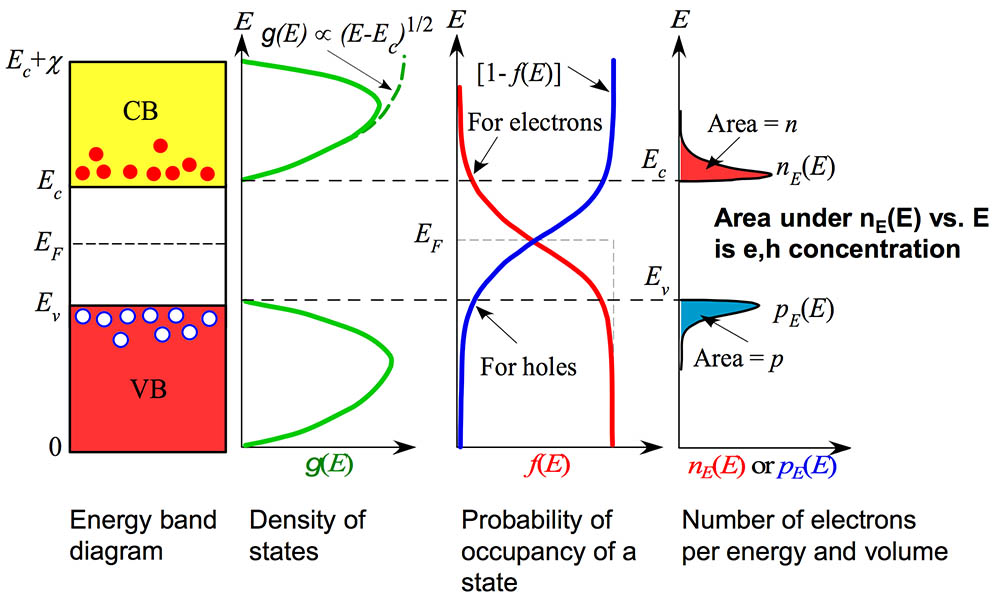
\includegraphics[width=0.6\linewidth]{images/semicond_elec_hole_concentration.jpg}
\end{figure}

The electron concentration $n$ and the hole concentration $p$ are calculated by
\begin{align}
    n &= N_C \cdot e^{-\frac{E_C-E_F}{k T}} && \text{with} & N_C &= 2 \left( \frac{2 \pi m_e^* k T}{h^2} \right)^{3/2} \\
    p &= N_V \cdot e^{-\frac{E_C-E_F}{k T}} && \text{with} & N_V &= 2 \left( \frac{2 \pi m_h^* k T}{h^2} \right)^{3/2}
\end{align}
where $N_C$ and $N_V$ are the effective densities of states at the CB edge and at the VB edge.

The \emph{mass action law} states that
\begin{equation}
    n p = n_i^2 = N_C N_V \cdot e^{-\frac{E_C-E_V}{k T}} = N_C N_V \cdot e^{-\frac{E_G}{k T}}
\end{equation}
where $n_i$ is the electron and hole concentration in an intrinsic semiconductor.

\begin{table}[hbp!]
    \centering
    \begin{tabular}{lll}
        $n = p$ & $\Rightarrow$ & intrinsic semiconductor \\
        $n > p$ & $\Rightarrow$ & n-type semiconductor \\
        $p > n$ & $\Rightarrow$ & p-type semiconductor \\
    \end{tabular}
\end{table}

The Fermi energy in an intrinsic semiconductor is
\begin{align}
    E_{Fi} &= E_V + \frac{1}{2} E_g - \frac{1}{2} k T \ln \frac{N_C}{N_V} \\
    &= E_V + \frac{1}{2} E_g - \frac{3}{4} k T \ln \frac{m_e^*}{m_h^*} \\
    &= E_V + \frac{1}{2} E_g \qquad \text{if} \quad m_e^*=m_h^* \:,\: N_C = N_V
\end{align}

The Fermi level is almost in the middle of the energy gap.
In Si and Ge, it is slightly below midgap.
%TODO: add image from 5.14


As $np = n_i^2$ must always be fulfilled,
\begin{align*}
    n \uparrow \;\Leftrightarrow\; E_F \uparrow && p \uparrow \;\Leftrightarrow\; E_F \downarrow
\end{align*}

The average energy of an electron in the conduction band is
\begin{equation}
    \bar{E}_{CB} = E_C + \frac{3}{2} kT
\end{equation}

\begin{figure}[htbp]
    \centering
    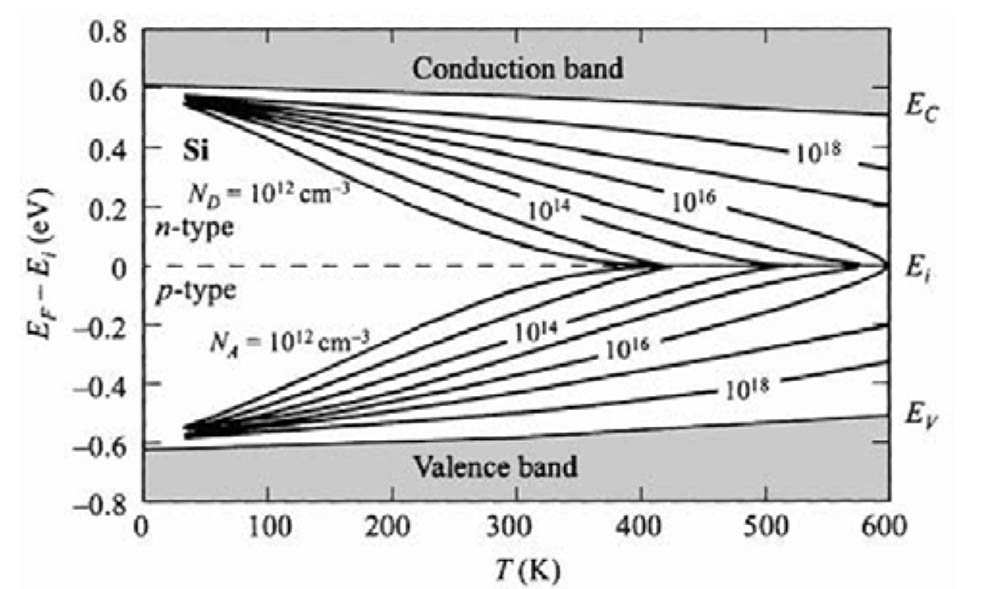
\includegraphics[width=0.6\linewidth]{images/semiconductors_fermi_energies.jpg}
    \caption{Fermi energy in silicon as a function of temperature and impurity concentration}
\end{figure}

The typical properties of some semiconductors is depicted in appendix~\ref{app:semiconductors}.

\subsection{Extrinsic semiconductors\buch{388}}
%TODO: bänder mit As und B einfügen, sowie formel verstehen + einfügen!--> kasap?
\paragraph{N-Type}
In n-type semiconductors, the impurity is a \emph{donor} atom, such as As, P, Sb.
This leads to an unbonded $e^-$ which orbits around the ionic center.
With $n \approx N_d$ (as $N_d \gg n_i$) this leads to
\begin{equation}
    \sigma \approx e N_d \mu_e
\end{equation}

\paragraph{P-Type}
In p-type semiconductors, the impurity is a \emph{acceptor} atom, such as B, Al, Ga, In.
This leads to a missing $e^-$ (hole) which orbits the negative site.
With $p \approx N_a$ (as $N_a \gg n_i$), this leads to
\begin{equation}
    \sigma \approx e N_a \mu_h
\end{equation}

\paragraph{Compensation doping}
is the situation in which a semiconductor contains both donors and acceptors.
Recombination takes place until either 
$n=N_d-N_a$ or $p=N_a-N_d$. 

\begin{align*}
    \text{More donors than acceptors:} && N_d - N_a &\gg n_i & n &= N_d - N_a & p &= \frac{n_i^2}{N_d-N_a} \\
    \text{More acceptors than donors:} && N_a - N_d &\gg n_i & n &= \frac{n_i^2}{N_a - N_d} & p &= N_a - N_d
\end{align*}

\subsection{Temperature dependence of conductivity\buch{396}}
The conductivity $\sigma = q n \mu $ where $n$ and $\mu$ are temperature dependant.

\begin{multicols}{3}
    \paragraph{Intrinsic range}
    $T > T_i$
    \begin{equation*}
        n = n_i \,\propto\, e^{\frac{E_g}{2kT}}
    \end{equation*}
    Intrinsic behavior \\
    Ionization across bandgap.
\vfill\columnbreak
    \paragraph{Extrinsic range}
    $T_s < T < T_i$
    \begin{equation*}
        n = N_d = \text{const.}
    \end{equation*}
    All donors ionized \\
    Electron conc. = donor conc.
\vfill\columnbreak    
    \paragraph{Ionization range}
    $T < T_s$
    \begin{equation*}
        n \,\propto\, e^{-\frac{\Delta E}{2kT}}
    \end{equation*}
    Donor ionization\\
     $T_s$: Saturation temperature.
\vfill
\end{multicols}

%TODO insert image from slide 21-23

\paragraph{Intrinsic carrier concentration}
The temperature dependence comes from the mass action law.
The slope is a measure of energy gap.
\begin{equation}
    n_i = \sqrt{np} = \sqrt{N_C N_V} e^{\frac{E_g}{2kT}}
\end{equation}

\paragraph{Drift mobility}
Scattering comes from \emph{impurities} at low temperatures 
($\mu \,\propto\, T^{+3/2}$) 
and from \emph{lattice vibrations} at high temperatures 
($\mu \,\propto\, T^{-3/2}$).
The drift mobility is 
\begin{equation}
    \mu = \frac{e \tau}{m_e^*}
\end{equation}
where $\tau$ is the mean free time between scattering events.
The mean free path $\lambda_{\textrm{mfp}}$ is
\begin{equation}
    \lambda_{\textrm{mfp}} = v_{th} \tau = \frac{1}{S N_S}
\end{equation}
where $S$ is the scattering cross-section, $N_S$ is the concentration of scatterers
and $v_{th}$ is the thermal velocity.

At high dopant concentrations, the electron and hole mobilities are limited
by impurity scattering.

\subsection{Direct and indirect recombination\buch{407,450}}
\begin{figure}[ht!]
    \centering
    \begin{tikzpicture}[>=latex]
\begin{scope}[shift={(-5,0)}]
    \begin{axis}[
        axis lines=middle, ticks=none, clip=false,
        domain=-pi:pi, samples=51,
        width=6cm, height=4cm,
        xmin=-pi, xmax=pi,
        ymin=0, ymax=6,
    ]
        % Plots
        \addplot[mark=none,black] {1.1+cos(deg(x))};
        \addplot[mark=none,black] {5-cos(deg(x))};
        
        % Text
        \node at (axis cs:-0.8,1) {VB};
        \node at (axis cs:-0.8,5) {CB};
    
        % Electrons
        \node[circle,draw=HSRBlue,fill=HSRBlue,inner sep=2] (e1) at (axis cs:0.1,4) {};
        \node[circle,draw=HSRBlue,fill=none,inner sep=2] (e2) at (axis cs:0.1,2.1) {};
        \draw[->] (e1) to (e2);
        
        % Photons
        \draw[->,HSRBlue,decorate,decoration={snake}] (axis cs:0.5,3.05) to (axis cs:2,3.05) node[anchor=west]{Photon};
    \end{axis}
\end{scope}
\begin{scope}[shift={(+5,0)}]
    \begin{axis}[
        axis lines=middle, ticks=none, clip=false,
        domain=-pi:pi, samples=51,
        width=6cm, height=4cm,
        xmin=-pi, xmax=pi,
        ymin=0, ymax=6,
    ]
        % Plots
        \addplot[mark=none,black] {1.1+cos(deg(x))};
        \addplot[mark=none,black] {4.5+cos(deg(1.5*x))};
        
        % Text
        \node at (axis cs:-0.8,1) {VB};
        \node at (axis cs:-1,5.5) {CB};
    
        % Electrons
        \node[circle,draw=HSRBlue,fill=HSRBlue,inner sep=2] (e1) at (axis cs:1.5,4) {};
        \node[circle,draw=HSRBlue,fill=none,inner sep=2] (e2) at (axis cs:0.1,2.1) {};
        \node[rectangle,draw,fill,minimum height=4,minimum width=8,inner sep=0] (er) at (axis cs:0.1,3.5) {};
        \draw[->] (e1) to (er);
        \draw[->] (er) to (e2);
        
        % Photons
        \draw[->,HSRBlue,decorate,decoration={snake}] (axis cs:0.8,4.0) to (axis cs:0.2,5.4);
        \draw[->,HSRBlue,decorate,decoration={snake}] (axis cs:0.5,2.8) to (axis cs:2,2.8) node[anchor=west]{Photons};
        
    \end{axis}
\end{scope}
\end{tikzpicture}
    \caption{Direct and indirect recombination in semiconductors}
\end{figure}
\begin{multicols}{2}
    \paragraph{Direct recombination} 
    Direct recombination happens through emission of photon,
    so no momentum transfer is required. 
    The high probability for recombination leads to a shorter carrier lifetime.
    Direct recombination is mainly used in optically active materials, e.g. GaAs for LEDs
    
    \paragraph{Indirect recombination}
    In Si and Ge recombination happens through recombination centers and thus
    takes up any momentum difference between $e$ and $h$.
    Due to the much lower likelihood, the carrier lifetime is longer.
    Indirect semiconductors are not suitable for optical applications.
\end{multicols}

\paragraph{Photogeneration}
When illumination a semiconductor with $h\nu > E_g$, electron-hole pairs are generated.
After the light is turned off, excess electrons and holes disappear by recombination.

The thermal equilibrium without illumination is
\begin{equation}
    n_{n0} p_{n0} = n_i^2
\end{equation}
The excess carrier concentration is $\Delta p_n = \Delta n_n$ which gives
a minority carrier concentration of $p_n = p_{n0} + \Delta p_n$.
The time evolution of excess minority carrier concentration is
\begin{align}
    \text{Change in excess hole concentration} &= \text{Photogeneration} - \text{Recombination} \notag \\
    \frac{d \Delta p_n}{dt} &= G_{ph} - \frac{\Delta p_n}{\tau_h}
\end{align}
where $\tau_h$ is the minority carrier lifetime. 

This leads to

\begin{align}
    \Delta p_n(t) &= \tau_h G_{ph} \left[ 1-e^{-\frac{t}{\tau_h}} \right] && \text{when switching on}\\
    \Delta p_n(t) &= \tau_h G_{ph} e^{-\frac{t}{\tau_h}} && \text{when switching off}    
\end{align}

\paragraph{Low level injection}
Low level injection in n-type semiconductors does not affect $n_n$, but drastically affects $p_n$
%TODO: but why???

\subsection{Optical absorption}
%TODO: was gits do dezue z schriibe?

\subsection{Schottky junction\buch{436}}

Important: $\Phi_m > \Phi_n$

\begin{figure}[ht!]
    \centering
    \begin{tikzpicture}[>=latex]

\begin{scope}[shift={(-5,0)}]
    \node at (3,5) {Before contact};

    % Metal
    \draw[draw=black,fill=HSRBlue] (0,0) rectangle (2,2);
    \draw[draw=black,fill=none] (0,2) rectangle (2,4);
    \node[anchor=south] at (1,4) {Metal};
    \node[anchor=east] at (0,2) {$E_{Fm}$};
    \draw[<->] (0.8,2) -- (0.8,4) node[midway,anchor=west] {$\Phi_m$};
    
    % Semiconductor
    \draw[draw=black,fill=HSRBlue] (4,0.5) rectangle (6,1.5);
    \draw[draw=black,fill=none] (4,2.5) rectangle (6,4);
    \node[anchor=south] at (5,4) {$n$-type semiconductor};
    \node[anchor=west] at (6,2.5) {$E_c$};
    \draw[dashed] (4,2.3) -- (6,2.3) node[anchor=north west] {$E_{Fn}$};
    \draw[<->] (4.8,2.3) -- (4.8,4) node[midway,anchor=west] {$\Phi_n$};
    
\end{scope}

\begin{scope}[shift={(+5,0)}]
    \node at (2,5) {After contact};

    % Metal
    \draw[draw=black,fill=HSRBlue] (0,0) rectangle (2,2);
    \draw[draw=black,fill=none] (0,2) rectangle (2,4);
    \node[anchor=east] at (0,2) {$E_{Fm}$};
    
    % Semiconductor
    \draw[draw=black,fill=none] (2,4) sin (2.5,3.7) -- (4,3.7) -- (4,2.2) -- (2.5,2.2) cos (2,2.5) -- (2,4);
    \draw[draw=black,fill=HSRBlue] (2,1.5) sin (2.5,1.2) -- (4,1.2) -- (4,0.2) -- (2.5,0.2) cos (2,0.5) -- (2,1.5);
    \node[anchor=west] at (4,2.2) {$E_c$};
    \draw[dashed] (2,2) -- (4,2) node[anchor=north west] {$E_{Fn}$};
    
    % Other stuff
    \draw[dashed] (1.5,2.5) -- (2.5,2.5);
    \draw[<->] (1.7,2) -- (1.7,2.5) node[midway,anchor=east] {$\Phi_B$};
    
\end{scope}

\end{tikzpicture}
    \caption{Schottky junction}
\end{figure}

From the CB to the metal, an $e^-$ tunnel is formed, which creates an $e^-$
depleted region in the semiconductor.
This built-in potential $V_0$ prevents a further flow of $e^-$.

\begin{equation}
    \Phi_B = \Phi_M - \chi = e V_0 + E_C - E_{Fn} > e V_0
\end{equation}

When applying a \emph{forward} bias, the electrons can easily overcome the small
barrier to enter the metal.
When applying a \emph{reverse} bias, the electrons in the metal cannot overcome
the barrier $\Phi_B$ to enter the semiconductor.

The Schottky junction is mainly used as diode. 
It is also possible to build Schottky solar cells ($h\nu>E_g$) and photo diodes.

\subsection{Ohmic contact\buch{443}}

Important: $\Phi_m < \Phi_n$

\begin{figure}[ht!]
    \centering
    \begin{tikzpicture}[>=latex]

\begin{scope}[shift={(-5,0)}]
    \node at (3,5) {Before contact};

    % Metal
    \draw[draw=black,fill=HSRBlue] (0,0) rectangle (2,3);
    \draw[draw=black,fill=none] (0,3) rectangle (2,4);
    \node[anchor=south] at (1,4) {Metal};
    \node[anchor=east] at (0,3) {$E_{Fm}$};
    \draw[<->] (0.8,3) -- (0.8,4) node[midway,anchor=west] {$\Phi_m$};
    
    % Semiconductor
    \draw[draw=black,fill=HSRBlue] (4,0.5) rectangle (6,1.5);
    \draw[draw=black,fill=none] (4,2.5) rectangle (6,4);
    \node[anchor=south] at (5,4) {$n$-type semiconductor};
    \draw[dashed] (4,2.3) -- (6,2.3) node[anchor=west] {$E_{Fn}$};
    \draw[<->] (4.8,2.3) -- (4.8,4) node[midway,anchor=west] {$\Phi_n$};
    
\end{scope}

\begin{scope}[shift={(+5,0)}]
    \node at (2,5) {After contact};

    % Metal
    \draw[draw=black,fill=HSRBlue] (0,0) rectangle (2,3);
    \draw[draw=black,fill=none] (0,3) rectangle (2,4);
    \node[anchor=east] at (0,3) {$E_{Fm}$};
    
    % Semiconductor
    \draw[draw=black,fill=none] (2,4) sin (2.5,4.5) -- (4,4.5) -- (4,3.2) -- (2.5,3.2) cos (2,2.7) -- (2,4);
    \draw[draw=black,fill=HSRBlue] (2,1.7) sin (2.5,2.2) -- (4,2.2) -- (4,1.2) -- (2.5,1.2) cos (2,0.7) -- (2,1.7);
    \draw[dashed] (2,3) -- (4,3) node[anchor=west] {$E_{Fn}$};
   
\end{scope}

\end{tikzpicture}
    \caption{Ohmic junction}
\end{figure}

An $e^-$ tunnel into the semiconductor is built, which leads to an $e^-$
accumulation in the semiconductor, near the junction. 
This prevents a further $e^-$ flow. 
There is no barrier for $e^-$ moving across the junction.

\paragraph{Peltier effect}
Current from SC into the metal results in a \emph{head absorption} at the junction,
which creates a \emph{cooling effect}.
Current from the metal into the SC results in a \emph{heat release} at the junction,
which creates a \emph{heating effect}.
